\begin{figure}[htp]
\centering
    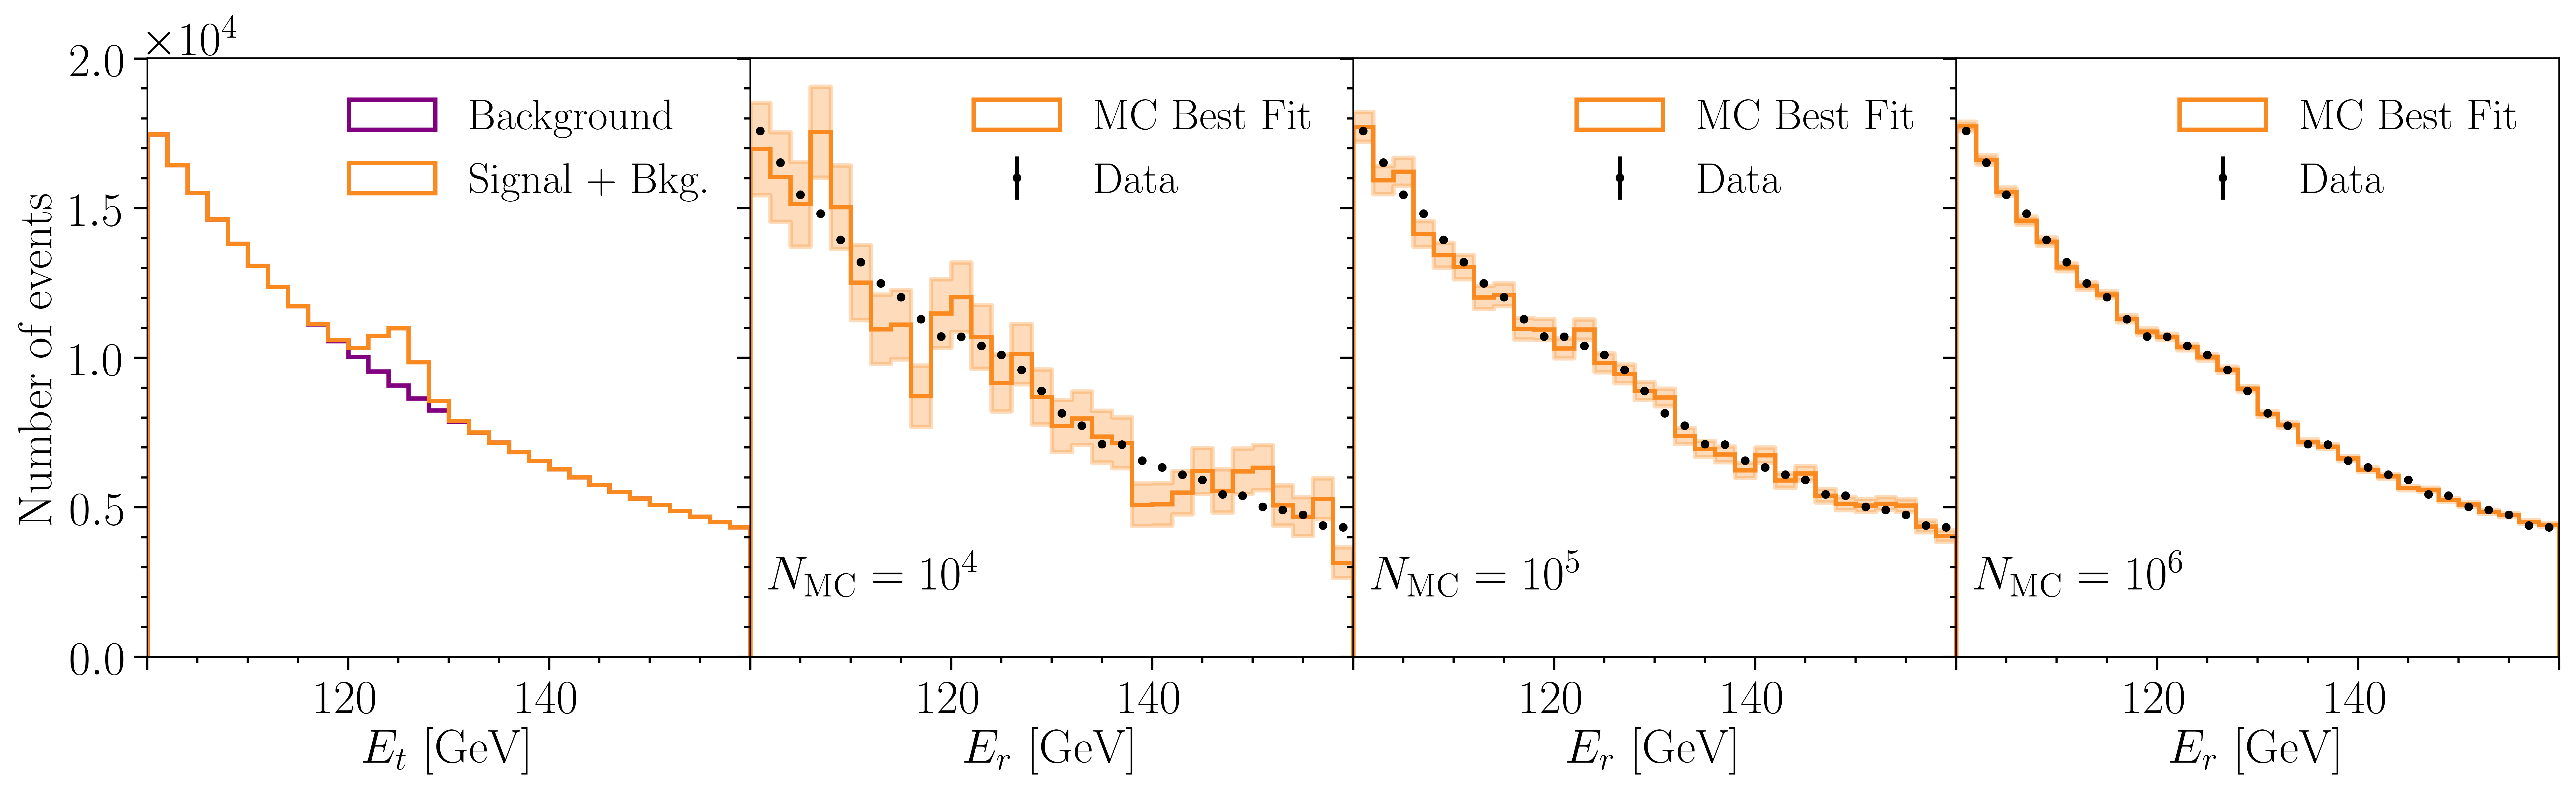
\includegraphics[width=1.\linewidth]{fig/fig4}
\caption{\textbf{\textit{Benchmark scenario.}} Leftmost panel: the underlying distribution that data is drawn from with background (purple) and total rate (orange).
Right three panels: observed data (black), $\mcl$ best-fit MC distributions (orange), and MC uncertainties (orange band), with increasing MC size from left to right.
The background component and signal width are fixed, while the mean and normalization of the signal peak are fit by maximizing the likelihood with respect to those parameters.}
\label{fig:toymc}
\end{figure}

Figure~\ref{fig:toymc} shows the expectation in $E_t$ as well as the data and $\mcl$ best-fit distributions in $E_r$.
The leftmost panel shows the expectation for both signal and background assuming no smearing in $E_t$.
The three other panels show the smeared, $E_r$, distribution for data (black) and the best-fit result from $\mcl$ for three different MC datasets (orange) of varying MC size.
The smeared shape of the signal peak is clearly visible in data, but not in the smallest size MC.
As the MC increases in size, the best-fit MC distribution can be seen to converge to the data distribution.

\begin{table}[htp]
\centering
\begin{tabular}{l r r r}
\toprule
Likelihood & $N_\mathrm{MC}=10^4$ & $10^5$ & $10^6$ \\
\midrule
%\hhline{ | = # = # = # = # = # = # = # = # = # = # = | }
$\adhoc$ & $(127.0,6368.0)$ & $(124.7,5655.7)$ & $(125.1,4888.5)$ \\ \hline
$\mcl$ & $(127.1,6077.1)$ & $(124.7,5576.0)$ & $(125.1,4889.4)$ \\
\bottomrule
\end{tabular}
\caption{\textbf{\textit{Best-fit parameters}} For the toy experiment shown in Fig.~\ref{fig:toymc}, best-fit parameters using $\adhoc$ and $\mcl$ are shown.
The columns in the table are for the different MC sizes.
The two numbers in parentheses for each entry correspond to $\Omega$ and $\Phi$, respectively.}
\label{tbl:pointestimator}
\end{table}

The best-fit values for the example shown in Fig.~\ref{fig:toymc} are given in Table~\ref{tbl:pointestimator} for $\mcl$ and $\adhoc$.
As point estimators, both likelihoods return similar values.
This is driven by the fact that the same underlying MC distribution is used to fit to the data.
The effect of convoluting $\prob(\lambda|\vecw(\vectheta))$ mostly serves to broaden the likelihood space, while preserving the maximum within the constraints described in Sec.~\ref{sec:llhbehavior}.
In the large MC limit, both likelihoods can be used for unbiased point estimation, provided that the likelihood space is smooth enough for standard minimization techniques to probe the global minimum.
